%\documentclass[12pt,aspectratio=169]{beamer}
%\input{../mybeamer}

\chapter{Mechanical Waves}
\label{chapter:waves}


A \textbf{mechanical wave} is a travelling disturbance that transports energy
through a medium.
\begin{figure}[ht]
  \centering
  \begin{tikzpicture}[scale=1.3]
    \node[mass-element] (m1) at (0,0) {$m$};
    \node[mass-element] (m2) at (2,0) {$m$};
    \node[mass-element] (m3) at (4,0) {$m$};
    \node[mass-element] (m4) at (6,0) {$m$};
    \node[mass-element] (mx) at (12,0) {$m$};
    \draw[springy] (m1)--(m2) node[midway,above=4]{$k$};
    \draw[springy] (m2)--(m3) node[midway,above=4]{$k$};
    \draw[springy] (m3)--(m4) node[midway,above=4]{$k$};
    \draw[springy] (m4)--(7.6,0) node[midway,above=4]{$k$};
    \draw[springy] (10.4,0)--(mx) node[midway,above=4]{$k$};
    \foreach \x in {8,8.25,...,10} \fill (\x,0) circle (.05);
  \end{tikzpicture}
  \caption{Model for a mechanical wave}
  \label{fig:wave-model}
\end{figure}
In this model of a wave, disturbance in the 1st mass causes the 1st spring to
displace, which causes motion in the 2nd masses, which causes the 2nd spring
to displace\ldots\footnote{This model is, in fact, how we derive the ``wave
equation'' that university students in math, physics and engineering have
to study.}
%
%
%
%
%{Mechanical Waves}
\begin{itemize}
\item When a disturbance (vibration) causes vibrations in its vicinity, a
  wave is created
\item A mechanical wave does not transport matter
\item Examples of mechanical waves:
  \begin{itemize}
  \item Sound wave (medium: air, solids and liquids)
  \item Ocean wave (medium: water)
  \item Wave on a string (medium: string, rope)
  \end{itemize}
\end{itemize}



%{Electromagnetic Waves}
In contrast, electromagnetic (''EM'') waves do not require a medium. EM waves
include:
\begin{itemize}
\item Radio waves
\item Microwave
\item Infrared radiation
\item Visible light
\item Ultraviolet radiation
\item X-ray
\item Gamma ray
\end{itemize}
%
%
%
%
%
%{Two Kinds of Waves}
%  \begin{center}
%    \pic{.6}{main-qimg}
%  \end{center}
%  \begin{enumerate}[a.]
%  \item\textbf{Longitudinal wave}
%    \begin{itemize}
%    \item Vibrations are parallel to the direction of the motion of the wave
%    \item Example: sound waves
%    \end{itemize}
%  \item\textbf{Transverse wave}
%    \begin{itemize}
%    \item Vibrations are perpendicular to the direction of the motion of the
%      wave
%    \item Example: electromagnetic waves
%    \end{itemize}
%  \end{enumerate}
%
%
\section{Properties of Waves}
%
%{Harmonic Wave}
\begin{itemize}
\item The \emph{highest} point\footnote{This is where the physical property
that defines the wave is at its maximum value.} of the wave is called a
  \textbf{crest} or \textbf{peak}, while
\item The \emph{lowest} point in the wave is called a \textbf{trough} or a
  \textbf{valley}
\item The \textbf{wavelength} $\lambda$ is the shortest distance between two
  points in the medium that are in phase. The easiest way to measure
  wavelength is from crest to crest, or from trough to trough
\end{itemize}

\begin{figure}[ht]
  \centering
  \begin{tikzpicture}
    \draw[thick] (0,0)--(12,0); % center line
    \draw[smooth,samples=60,domain=0:12,functions]
    plot(\x,{sin(60*(\x-1))}); % the wave itself
    \draw[vectors,red] (5,.6)--(6,.6)
    node[midway,above,black!80]{Direction of wave travel};
    \begin{scope}[<->] % arrow quantities
      \draw (2.5,1)--(2.5,0) node[midway,fill=black!2]{$A$};
      \draw (5.5,-1)--(5.5,0) node[midway,fill=black!2]{$A$};
      \draw (2.5,1.5)--(8.5,1.5) node[midway,fill=black!2]{$\lambda$};
      \draw (5.5,-1.5)--(11.5,-1.5)node[midway,fill=black!2]{$\lambda$};
    \end{scope}
    \draw (2.5,1.7)--(2.5,1) node[above]{Crest};
    \draw (8.5,1.7)--(8.5,1) node[above]{Crest};
    \draw (5.5,-1.7)--(5.5,-1) node[below]{Trough};
    \draw (11.5,-1.7)--(11.5,-1) node[below]{Trough};
  \end{tikzpicture}
\end{figure}


%{Pulse Wave}
A wave can also be defined as a single pulse:
\begin{figure}[ht]
  \centering
  \begin{tikzpicture}[functions]
    \draw (-5,0)--(-2,0);
    \draw (2,0)--(5,0);
    \draw[smooth,samples=30,domain=-2:2] plot(\x,{3*exp(-\x*\x/.05)});
    \draw[->] (1,.6)--(2,.6) node[right,black!80]{Dir.\ of wave travel};
  \end{tikzpicture}
\end{figure}
The wavelength $\lambda$ of a pulse wave is \emph{undefined} because no two
points are in phase.
%
%
%
%
%\section{Wave Equation}
%
%{The Wave Equation}
%  The mechanical wave as we know it is the solution to a second-order partial
%  differential equation, subject to initial and boundary conditions:
%  
%  \eq{-.1in}{
%    \frac{\partial^2 u}{\partial t^2} = v^2\frac{\partial^2 u}{\partial x^2}
%  }
%
%  This is a type of equation that is taught in third year of university (i.e.\
%  not necessary to know right now)
%
%
%
%
%{Equation of a Travelling Wave}
%  One solution to the wave equation is a \textbf{harmonic wave} that can be
%  described as a sinusoidal function that oscillates in both space $x$ and time
%  $t$:
%  
%  \eq{-.1in}{
%    \boxed{u(x,t)=A\sin(kx-\omega t)}
%  }
%  \begin{center}
%    \begin{tabular}{l|c|c}
%      \rowcolor{pink}
%      \textbf{Quantity} & \textbf{Symbol} & \textbf{SI Unit} \\ \hline
%      Displacement of the medium  & $u$ & \si\metre \\
%      Amplitude of the wave       & $A$ & \si\metre \\
%      Wave number                 & $k$ & \si{\per\metre} \\
%      Distance from the source    & $x$ & \si\metre \\
%      Time                        & $t$ & \si\second \\
%      Angular frequency           & $\omega$ & \si{rad\per\second}
%    \end{tabular}
%  \end{center}
%  Displacement $u$ is measured from the rest position
%
%
%
%
%
%{Equation of a Travelling Wave}
%  \eq{-.1in}{
%    \boxed{u(x,t)=A\sin(kx-\omega t)}
%  }
%
%  The angular frequency is related to the frequency $f$ and period $T$ of the
%  wave by:
%
%  \eq{-.1in}{
%    \omega=\frac{2\pi}T=2\pi f
%  }
%
%  The \textbf{wave number} $k$ is the \emph{spatial frequency} of the wave, and
%  is related to the wavelength $\lambda$ by:
%  
%  \eq{-.1in}{
%    k=\frac{2\pi}\lambda
%  }
%
%
%
%
%{Speed of a Wave}
%  The speed of \emph{any} wave can be related to the wave number and angular
%  frequency by:
%
%  \eq{-.1in}{
%    v=\frac\omega k=\frac{2\pi f}{2\pi/\lambda}\quad\rightarrow\quad
%    \boxed{v=f\lambda=\frac\lambda T}
%  }
%  \begin{center}
%    \begin{tabular}{l|c|c}
%      \rowcolor{pink}
%      \textbf{Quantity} & \textbf{Symbol} & \textbf{SI Unit} \\ \hline
%      Speed             & $v$       & \si{\metre\per\second} \\
%      Wave number       & $k$       & \si{\per\metre} \\
%      Angular frequency & $\omega$  & \si{\radian\per\second}\\
%      Frequency         & $f$       & \si\hertz \\
%      Wavelength        & $\lambda$ & \si\metre \\
%      Period            & $T$       & \si\metre 
%    \end{tabular}
%  \end{center}
%
%
%
%
%\subsection%{Wave on a String}
%  The speed of a travelling wave on a stretched string is determined by:
%  
%  \eq{-.1in}{
%    \boxed{v=\sqrt{\frac T\mu}}
%    \quad\text{\normalsize where}\quad
%    \boxed{\mu=\frac mL}
%  }
%  \begin{center}
%    \begin{tabular}{l|c|c}
%      \rowcolor{pink}
%      \textbf{Quantity} & \textbf{Symbol} & \textbf{SI Unit} \\ \hline
%      Wave speed           & $v$   & \si{\metre\per\second} \\
%      Tension              & $T$   & \si\newton \\
%      Linear mass density  & $\mu$ & \si{\kilo\gram\per\metre} \\
%      Mass of the string   & $m$   & \si{\kilo\gram} \\
%      Length of the string & $L$   & \si\metre
%    \end{tabular}
%  \end{center}
%
%
%
%
%{Frequency and Speed of A Wave}
Frequency ($f$) of a wave:
\begin{itemize}
\item The number of complete wavelengths that pass a point in a given amount
  of time
\item Same as the frequency of the disturbance that generated the wave
\item\textbf{Depends only on the source}, not the medium
\end{itemize}

Speed ($v$) of a travelling wave:
\begin{itemize}
\item The speed at which the wave fronts are moving
\item \textbf{Depends only on the medium}, not the source disturbance that
  produced the wave
\end{itemize}




\section{Harmonic Waves}
%
%{Fourier Series}
Not all harmonic waves have to have a sinusoidal shape, because \emph{all}
periodic functions with (spatial) period $P$ (related to the wavelength) are
actually infinite sums of sine and/or cosine functions, called the
\textbf{Fourier series}:
\begin{align*}
  u(x)=\frac{a_0}2 + 
  \sum_{n=1}^\infty a_n\sin\left(\frac{2\pi n}Px\right)+
  \sum_{n=1}^\infty b_n\cos\left(\frac{2\pi n}Px\right)
\end{align*}
Depending on the shape of the harmonic wave, some coefficients $a_n$ and $b_n$
are zeros.

For example, this harmonic wave is a composite of 4 sine waves all travelling
at the same speed. (The coefficients are arbitrarily chosen.)
{\footnotesize
  \begin{displaymath}
    u(x)=\sin(50x)+\frac25\sin(100x) +\frac1{10}\sin(150x)
    +\frac15\sin(200x) +\frac3{10}\sin(250x)
  \end{displaymath}
}
\begin{center}
  \begin{tikzpicture}[xscale=.4]
    \draw[thick] (-1,0)--(21,0);
    \draw[smooth,samples=500,domain=-1:21,very thick,red]
    plot(\x, {sin(50*\x)+.4*sin(100*\x)+.1*sin(150*\x)
      +.2*sin(200*\x)+.3*sin(250*\x)});
    \draw[<->] (7.75,1.5)--(14.9,1.5)
    node[midway,fill=black!2]{$\lambda$};
    \draw[vectors,red] (22,.6)--(25,.6)
    node[midway,above,black!80]{Direction of wave travel};
  \end{tikzpicture}
\end{center}




%{Fourier Series and Harmonic Frequencies}
%  \begin{center}
%    \begin{tikzpicture}
%      \draw[thick] (0,0) --(3,0);
%      \draw[vectors] (1,1.3)--(1.5,1.3) node[right]{$v$};
%      \draw[thick,cyan,smooth,samples=80,domain=0:2.8] plot(\x,{sin(200*\x)});
%      \node[below] at (1.5,-1.3){Fundamental};
%    \end{tikzpicture}
%    \hspace{.15in}
%    \begin{tikzpicture}
%      \draw[thick] (0,0) --(3,0);
%      \draw[vectors] (1,1.3)--(1.5,1.3) node[right]{$v$};
%      \draw[thick,magenta,smooth,samples=80,domain=0:2.8]
%      plot(\x,{sin(400*\x)});
%      \node[below] at (1.5,-1.3){2nd Harmonic};
%    \end{tikzpicture}
%    \hspace{.15in}
%    \begin{tikzpicture}
%      \draw[thick] (0,0) --(3,0);
%      \draw[vectors] (1,1.3)--(1.5,1.3) node[right]{$v$};
%      \draw[thick,violet,smooth,samples=80,domain=0:2.8] plot(\x,{sin(600*\x)});
%      \node[below] at (1.5,-1.3){3rd Harmonic};
%    \end{tikzpicture}
%  \end{center}
%  \begin{itemize}
%  \item The wave with the longest wavelength (therefore lowest frequency) is
%    called the \textbf{fundamental frequency}, or \textbf{first harmonic}
%  \item The second wave has half the wavelength and twice the frequency. It's
%    called the \textbf{second harmonic}, or the \textbf{first overtone}
%  \item Also, third, fourth, fifth\ldots harmonics
%  \end{itemize}
%  These terms are also used by musicians when it is related to sound waves.
%
%
%
%
%{Harmonic Frequencies}
%  Whole-number multiples of the fundamental frequency $f_1$ are its
%  harmonic frequency, i.e.\ the $n$-th harmonic is:
%
%  \eq{-.1in}{
%    \boxed{f_n=nf_1}\quad n=1,2,3,\ldots
%  }
%  
%  %For sound waves, when a musical instrument produces a sound that has many
%  %harmonics, the frequency that is ``heard'' is the fundamental frequency
%
%
%
%
%{Wave Simulation}
%  A helpful simulation can be found on the PhET website at University of
%  Colorado.
%  \begin{center}
%    \textbf{Click for external link:}\\
%    \href{https://phet.colorado.edu/sims/html/wave-on-a-string/latest/wave-on-a-string_en.html}
%         {wave on a string simulation}
%  \end{center}
%
%
%
%
%{Power Transmitted by a Harmonic Wave}
%  The average power $P$ transmitted by a harmonic wave on a string is given by:
%
%  \eq{-.1in}{
%    \boxed{P=\frac12\mu\omega^2A^2v}
%  }
%  \begin{center}
%    \begin{tabular}{l|c|c}
%      \rowcolor{pink}
%      \textbf{Quantity} & \textbf{Symbol} & \textbf{SI Unit} \\ \hline
%      Average power       & $P$ & \si\watt \\
%      Linear mass density & $\mu$    & \si{\kilo\gram\per\metre}\\
%      Angular frequency   & $\omega$ & \si{\radian\per\second}\\
%      Wave amplitude      & $A$      & \si\metre \\
%      Wave speed          & $v$      & \si{\metre\per\second}
%    \end{tabular}
%  \end{center}  
%
%
%
%
%{Intensity of a 3D Wave}
%  For three dimension waves (e.g.\ sound waves), the wavefront expands as the
%  wave propagates forward. It is more convenient to describe the
%  power transmitted by its \textbf{intensity} $I$:
%
%  \eq{-.1in}{
%    \boxed{I=\frac PS}
%  }
%
%  For a spherical wave (e.g.\ sound emitted from a stationary source), the area
%  that the wavefront passes through is $S=4\pi r^2$, where $r$ is the distance
%  from the source.

\section{Reflection of a Wave at a Boundary}

When a wave on a string reflects at a boundary, how the reflected wave looks
depends on the type of boundary
\begin{itemize}
\item At a \emph{fixed end} (left):
  \begin{itemize}
  \item the reflected wave is \emph{inverted}
  \item i.e.\ a phase shift of $\pi$
  \item i.e.\ a crest becomes a trough
  \end{itemize}
\item At a \emph{free end} (right)
  \begin{itemize}
  \item the reflected wave is upright
  \item No phase shifts
  \end{itemize}
\end{itemize}
\begin{center}
  \pic{.5}{mechanicalWaves/22}
\end{center}

\section{Transmission of Waves}
%: Fast to Slow Medium}
%  \begin{columns}
%    \column{.6\textwidth}
%    \begin{itemize}
%    \item Reflected wave:
%      \begin{itemize}
%      \item Inverted, like a fixed end
%      \item Same frequency and wavelength as the incoming wave
%      \item The amplitude is decreased because energy is split between the
%        reflected and transmitted waves
%      \end{itemize}
%    \item Transmitted wave:
%      \begin{itemize}
%      \item Upright
%      \item Same frequency as incoming wave, but has a shorter wavelength
%        because the wave slowed down
%      \end{itemize}
%    \end{itemize}
%    
%    \column{.4\textwidth}
%    \pic1{23}
%  \end{columns}
%
%
%
%{Transmission of Waves: Slow to Fast Medium}
%  \begin{columns}
%    \column{.6\textwidth}
%    \begin{itemize}
%    \item Reflected wave:
%      \begin{itemize}
%      \item Upright, like a free end
%      \item Same frequency and wavelength as the incoming wave
%      \item The amplitude is decreased because energy is split between the
%        reflected and transmitted waves
%      \end{itemize}
%    \item Transmitted wave:
%      \begin{itemize}
%      \item Upright
%      \item Same frequency as incoming wave, but has a longer wavelength because
%        the wave sped up
%      \end{itemize}
%    \end{itemize}
%    
%    \column{.4\textwidth}
%    \pic1{24}
%  \end{columns}
%  
%  \vspace{.1in}Note that the transmitted wave is \emph{always} upright.
%
%
%
%
\section{Wave Interference}
%
%{Superposition of Waves}
%  \begin{center}
%    \pic{.6}{omkAt}
%  \end{center}
\begin{itemize}
\item\textbf{Principle of Superposition:} When multiple waves pass through
  the same point, the resultant wave is the \emph{sum} of the waves
  \begin{itemize}
  \item A fancy way of saying that waves add together
  \end{itemize}
\item The consequence of the principle of superposition is
  \textbf{interference of waves}. There are two kinds of interference:
  \begin{itemize}
  \item\textbf{Constructive interference:} Two wave fronts (crests) passing
    through creates a wave front with greater amplitude
  \item\textbf{Destructive interference:} A crest and trough will cancel
    each other
  \end{itemize}
\end{itemize}




\subsection{Constructive Interference}
%  \vspace{.1in}
\begin{center}
  \begin{tikzpicture}[scale=.8]
    \draw[cyan,very thick,domain=-3:3,smooth,samples=120]
    plot(\x,{exp(-3*(\x-1.5)^2)+exp(-3*(\x+1.5)^2)});
    \draw[vectors,red!70!black] (-1.8,.4)--(-1.2,.4);
    \draw[vectors,red!70!black] (1.8,.4)--(1.2,.4);
  \end{tikzpicture}
  \hspace{.2in}
  \begin{minipage}{.6\textwidth}
    \vspace{-.3in}
    \small Two pulse waves (shown as crests), one travelling to the right,
    and the other one to the left. At this time, the two waves do
    not interact.\par
  \end{minipage}

  \vspace{.2in}
  \begin{tikzpicture}[scale=.8]
    \begin{scope}[very thick,smooth]
      \draw[cyan!30,domain=-2:2,samples=120] plot(\x,{exp(-3*(\x-.5)^2)});
      \draw[cyan!30,domain=-2:2,samples=120] plot(\x,{exp(-3*(\x+.5)^2)});
      \draw[cyan,domain=-3:3,samples=120]
      plot(\x,{exp(-3*(\x-.5)^2)+exp(-3*(\x+.5)^2)});
    \end{scope}
    \draw[vectors,red!70!black] (-.8,.4)--(-.2,.4);
    \draw[vectors,red!70!black] (.8,.4)--(.2,.4);
  \end{tikzpicture}
  \hspace{.2in}
  \begin{minipage}{.6\textwidth}
    \vspace{-.3in}
    \small As the two waves begin to overlap, the parts where the waves
    overlap is the superposition (sum) of the waves.\par
  \end{minipage}

  \vspace{.15in}
  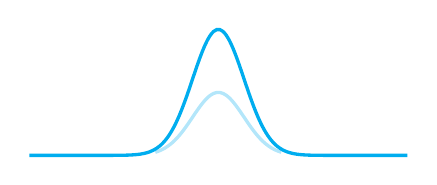
\begin{tikzpicture}[scale=.8]
    \begin{scope}[very thick,smooth]
      \draw[cyan!30,domain=-1:1,samples=40] plot(\x,{exp(-3*(\x)^2)});
      \draw[cyan,domain=-3:3,samples=120] plot(\x,{2*exp(-3*(\x)^2)});
    \end{scope}
  \end{tikzpicture}
  \hspace{.2in}
  \begin{minipage}{.6\textwidth}
    \vspace{-.65in}
    \small For a brief moment, the two waves completely overlap each other,
    resulting in an amplitude greater than each of the two crests.
    This is called \textbf{constructive interference}.\par
  \end{minipage}

  \vspace{.2in}
  \begin{tikzpicture}[scale=.8]
    \draw[cyan,very thick,domain=-3:3,smooth,samples=120]
    plot(\x,{exp(-3*(\x-1.5)^2)+exp(-3*(\x+1.5)^2)});
    \draw[vectors,red!70!black] (-1.2,.4)--(-1.8,.4);
    \draw[vectors,red!70!black] (1.2,.4)--(1.8,.4);
  \end{tikzpicture}
  \hspace{.2in}
  \begin{minipage}{.6\textwidth}
    \vspace{-.2in}
    \small After the two waves have pass through each other, they continue to
    travel along the medium \emph{as if no interaction had occured}.\par
  \end{minipage}   
\end{center}
%
%
%
%
\subsection{Destructive Interference}
%  \vspace{.1in}
%  \begin{center}
%    \begin{tikzpicture}[scale=.8]
%      \draw[cyan,very thick,domain=-3:3,smooth,samples=120]
%      plot(\x,{-exp(-2.7*(\x-1.5)^2)+exp(-2.7*(\x+1.5)^2)});
%      \draw[vectors,red!70!black] (-1.8,.4)--(-1.2,.4);
%      \draw[vectors,red!70!black] (1.8,-.4)--(1.2,-.4);
%    \end{tikzpicture}
%    \hspace{.2in}
%    \begin{minipage}{.6\textwidth}
%      \vspace{-.7in}
%      \small Two pulse waves (one shown as a crest, the other as a trough),
%      travel towards each other. At this time, the two waves do
%      not interact.\par
%    \end{minipage}
%
%    \begin{tikzpicture}[scale=.8]
%      \begin{scope}[very thick,smooth]
%        \draw[cyan!30,domain=-2:2,samples=120] plot(\x,{-exp(-3*(\x-.3)^2)});
%        \draw[cyan!30,domain=-2:2,samples=120] plot(\x,{exp(-3*(\x+.3)^2)});
%        \draw[cyan,domain=-3:3,samples=120]
%        plot(\x,{-exp(-2.7*(\x-.3)^2)+exp(-2.7*(\x+.3)^2)});
%      \end{scope}
%      \draw[vectors,red!70!black] (-.8,.4)--(-.2,.4);
%      \draw[vectors,red!70!black] (.8,-.4)--(.2,-.4);
%    \end{tikzpicture}
%    \hspace{.2in}
%    \begin{minipage}{.6\textwidth}
%      \vspace{-.6in}
%      \small As the two waves overlap, we see the superposition (sum) of the
%      waves. Amplitudes begin to decrease as the two waves cancel
%      each other.\par
%    \end{minipage}
%
%    \vspace{.1in}
%    \begin{tikzpicture}[scale=.8]
%      \begin{scope}[very thick,smooth]
%        \draw[cyan!30,domain=-1:1,samples=40] plot(\x,{exp(-2.7*(\x)^2)});
%        \draw[cyan!30,domain=-1:1,samples=120] plot(\x,{-exp(-2.7*(\x)^2)});
%      \end{scope}
%      \draw[very thick,cyan] (-3,0)--(3,0);
%    \end{tikzpicture}
%    \hspace{.2in}
%    \begin{minipage}{.6\textwidth}
%      \vspace{-.65in}
%      \small For a brief moment, the two waves completely overlap,
%      resulting in the complete cancellation of the waves. This is called
%      \textbf{destructive interference}.\par
%    \end{minipage}
%
%    
%    \begin{tikzpicture}[scale=.8]
%      \draw[cyan,very thick,domain=-3:3,smooth,samples=120]
%      plot(\x,{exp(-2.7*(\x-1.5)^2)-exp(-2.7*(\x+1.5)^2)});
%      \draw[vectors,red!70!black] (-1.2,-.4)--(-1.8,-.4);
%      \draw[vectors,red!70!black] (1.2,.4)--(1.8,.4);
%    \end{tikzpicture}
%    \hspace{.2in}
%    \begin{minipage}{.6\textwidth}
%      \vspace{-.6in}
%      \small After the two waves have pass through each other, they continue to
%      travel along the medium \emph{as if no interaction had occured}.\par
%    \end{minipage}   
%  \end{center}
%
%
%
%
\section{Standing Waves}

Two identical waves (blue \& yellow) move in opposite directions in the same
medium. At some moment in time, they are out of phase, resulting in destructive
interference (green):
\begin{center}
  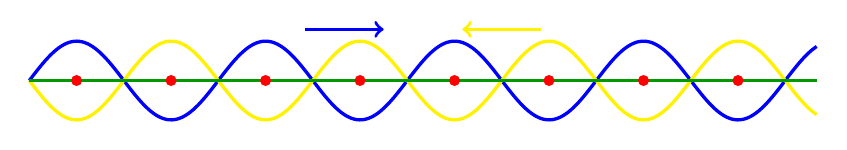
\begin{tikzpicture}[very thick]
    \draw[->,blue] (3.5,.65)--(4.5,.65);
    \draw[->,yellow] (6.5,.65)--(5.5,.65);
    \draw[smooth,samples=150,domain=0:10,blue] plot(\x,{.5*sin(150*\x)});
    \draw[smooth,samples=150,domain=0:10,yellow] plot(\x,{-.5*sin(150*\x)});
    \draw[green!60!black](0,0)--(10,0);
    \foreach \x in {0.6,1.8,...,10} \fill[red](\x,0) circle(.07);
  \end{tikzpicture}
\end{center}
A quarter of a wavelength later, the 2 waves are in phase (constructive
interference):
\begin{center}
  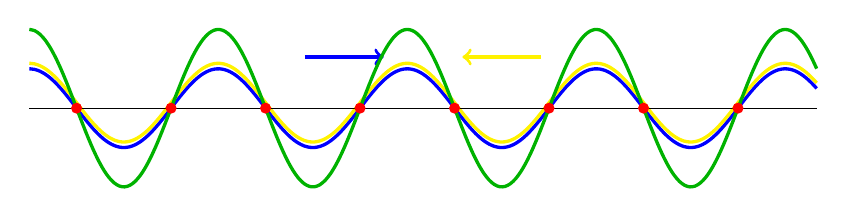
\begin{tikzpicture}[very thick]
    \draw[->,blue] (3.5,.65)--(4.5,.65);
    \draw[->,yellow] (6.5,.65)--(5.5,.65);
    \draw[smooth,samples=150,domain=0:10,blue]
    plot(\x,{.5*sin(150*\x+90)});
    \draw[smooth,samples=150,domain=0:10,yellow]
    plot(\x,{-.5*sin(150*\x-90)+0.07});
    \draw[smooth,samples=150,domain=0:10,green!70!black]
    plot(\x,{sin(150*\x+90)});
    \draw[thin] (0,0)--(10,0);
    \foreach \x in {.6,1.8,...,10} \fill[red] (\x,0) circle (.07);
  \end{tikzpicture}
\end{center}
But regardless of whether the wave is in phase, the red dots always have zero
displacement. They are called \textbf{nodes}.
%
%
%
%
%{Standing Waves}
If two waves of the same frequency meet up under the right conditions, they
may appear to be ``standing still''. This is called a \textbf{standing wave}.
\begin{center}
  \begin{tikzpicture}[scale=.7]
    \foreach \A in {-1.2,-1.1,...,1.2}
    \draw[cyan!60,smooth,samples=100,domain=0:12] plot(\x,{\A*sin(60*\x)});
    \draw[functions,smooth,samples=100,domain=0:12] plot(\x,{.7*sin(60*\x)});
    \draw (0,0)--(12,0);
    \draw (3,0)--+(-.3,-1.8)--+(-.6,-1.8) node[left]{node};
    \draw (9,0)--+(.3,-1.8)--+(.6,-1.8) node[right]{node};
    \draw (1.5,1.2)--+(.3,.5)--+(.6,.5) node[right]{anti-node};
    \draw (10.5,1.2)--+(.3,.5)--+(.6,.5) node[right]{anti-node};
    %\draw[|<->|] (4.5,-1.4)--+(3,0) node[midway,fill=white]{$\frac\lambda2$};
    %\draw[<->] (6,1.75)--+(3,0) node[midway,fill=white]{$\frac\lambda2$};
    %\draw (6,0)--+(0,1.85);
    %\draw (9,0)--+(0,1.85);
  \end{tikzpicture}
\end{center}
In a standing wave, the wavefronts do not move.
%(the location of the nodes and anti-nodes are fixed}.
Instead, you only see the medium vibrate. While it appears as if there
are \emph{no} waves travelling, there are, in fact, always \emph{two} waves
travelling in opposite directions.




%{Standing Waves}
%  \begin{center}
%    \begin{tikzpicture}[scale=.7]
%      \foreach \A in {-1.2,-1.1,...,1.2}
%      \draw[cyan!60,smooth,samples=100,domain=0:12] plot(\x,{\A*sin(60*\x)});
%      \draw[functions,smooth,samples=100,domain=0:12] plot(\x,{.7*sin(60*\x)});
%      \draw (0,0)--(12,0);
%      \draw (3,0)--+(-.3,-1.8)--+(-.6,-1.8) node[left]{node};
%      \draw (9,0)--+(.3,-1.8)--+(.6,-1.8) node[right]{node};
%      \draw (1.5,1.2)--+(.3,.5)--+(.6,.5) node[right]{anti-node};
%      \draw (10.5,1.2)--+(.3,.5)--+(.6,.5) node[right]{anti-node};
%      \draw[|<->|] (4.5,-1.4)--+(3,0)node[midway,fill=black!2]{$\frac\lambda2$};
%      \draw[<->] (6,1.75)--+(3,0) node[midway,fill=black!2]{$\frac\lambda2$};
%      \draw (6,0)--+(0,1.85);
%      \draw (9,0)--+(0,1.85);
%    \end{tikzpicture}
%  \end{center}
\begin{itemize}
\item Node: A point that never moves
\item Anti-node: A point which moves/vibrates maximally
\end{itemize}
Nodes and anti-nodes are evenly spaced.
%
%
%
%
%
\section{Standing Waves On a String}% of Length $L$}
\begin{itemize}
\item A ``vibrating'' string is actually a standing wave on a string
\item Both ends of the string are nodes
  %\item As the string vibrates, the air around it vibrates at the same frequency
  %\item The vibration travels as a sound wave toward your ears
  %\item Examples:
  %  \begin{itemize}
  %  \item Plucking a guitar or violin string
  %  \item Hitting a key on a piano/harpsichord
  %  \end{itemize}
\end{itemize}
%
%
%
%
%{Standing Waves On a String of Length $L$}
\textbf{Resonance modes} are frequencies where a standing wave can be
created. The first resonance (fundamental) frequency at occurs when
$\lambda=2L$, where $L$ is the length of the string. The ends of the strings
are nodes because they cannot vibrate
\begin{center}
  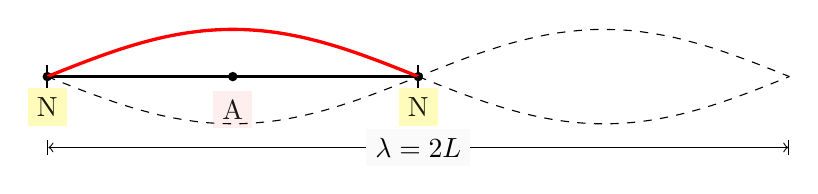
\begin{tikzpicture}[scale=1.5]
    \draw[thick] (0,0)--(pi,0);
    \draw[thick] (0,-.1) --(0,.1);
    \draw[thick] (pi,-.1)--(pi,.1);
    \draw[|<->|] (0,-.6)--(2*pi,-.6) node[midway,fill=black!2]{$\lambda=2L$};
    \foreach\x in {0,pi}
    \fill (\x,0) circle (.04) node[below=4,fill=yellow!30,opacity=.9]{N};
    \fill (pi/2,0) circle (.04) node[below=5,fill=pink!30,opacity=.9]{A};
    \begin{scope}[smooth,samples=20]
      \draw[domain=0:pi,red,very thick] plot(\x,{.4*sin(180/pi*\x)});
      \draw[domain=pi:2*pi,dashed] plot(\x,{.4*sin(180/pi*\x)});
      \draw[domain=0:2*pi,dashed] plot(\x,{-.4*sin(180/pi*\x)});
    \end{scope}
  \end{tikzpicture}
\end{center}
The fundamental frequency $f_1$ can be calculated based on the
speed of the travelling wave along the string $v$:
\begin{important-equation}
  f_1 = \frac v\lambda=\frac v{2L}
  \quad\text{\normalsize where}\quad
  v=\sqrt{\frac{F_T}\mu}
\end{important-equation}




%{Standing Waves On a String of Length $L$}
The second resonance mode ($n=2$) occurs when $\lambda=L$:

\begin{center}
  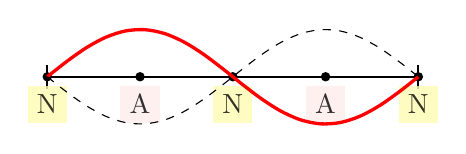
\begin{tikzpicture}[scale=1.5]
    \draw[thick] (0,0)--(pi,0);
    \draw[thick] (0,-.1)--(0,.1);
    \draw[thick] (pi,-.1)--(pi,.1);
    \foreach \x in {0,pi/2,pi}
    \fill (\x,0) circle (.04) node[below=3,fill=yellow!30,opacity=.8]{N};
    \foreach \x in {pi/4,3*pi/4}
    \fill (\x,0) circle (.04) node[below=3,fill=pink!30,opacity=.8]{A};
    \begin{scope}[smooth,samples=20,domain=0:pi]
      \draw[red,very thick] plot(\x,{.4*sin(360/pi*\x)});
      \draw[dashed] plot(\x,{-.4*sin(360/pi*\x)});
    \end{scope}
  \end{tikzpicture}
\end{center}

\begin{important-equation}
  f_2 = \frac v\lambda=\frac vL=2f_1
\end{important-equation}

%  \vspace{.2in}while the third resonance mode ($n=3$) occurs at
%  $\lambda=\dfrac23L$:
%  \begin{columns}
%    \column{.4\textwidth}
%    \centering
%    \begin{tikzpicture}[scale=1.5]
%      \draw[thick] (0,0)--(pi,0);
%      \draw[thick] (0,-.1)--(0,.1);
%      \draw[thick] (pi,-.1)--(pi,.1);
%      \foreach \x in {0,pi/3,2*pi/3,pi}
%      \fill (\x,0) circle (.04) node[below=4,fill=yellow!30,opacity=.9]{N};
%      \foreach \x in {pi/6,pi/2,5*pi/6}
%      \fill (\x,0) circle (.04) node[below=3,fill=pink!30,opacity=.8]{A};
%      \begin{scope}[smooth,samples=30,domain=0:pi]
%        \draw[red,very thick] plot(\x,{.4*sin(540/pi*\x)});
%        \draw[dashed] plot(\x,{-.4*sin(540/pi*\x)});
%      \end{scope}
%    \end{tikzpicture}
%    
%    \column{.6\textwidth}
%    \eq{-.01in}{
%      f_3=\frac v\lambda=\frac{3v}{2L}=3f_1
%    }
%  \end{columns}
%
%
%
%
%{Standing Waves On a String of Length $L$}
%  The $n$-th resonance mode of a wave on string is given by:
%
%  \eq{-.1in}{
%    \boxed{f_n=nf_1}\quad
%    \text{\normalsize where}\quad
%    \boxed{f_1=\frac v{2L}}
%  }
%  \begin{itemize}
%  \item $n=1,2,3,\ldots$ is a whole-number multiple
%  \item This equation is \emph{identical} to the equation for harmonic
%    frequencies, meaning that on a string, every harmonic is a resonance
%    frequency
%  \item A vibrating string is said to have a ``full set of harmonics''
%  \end{itemize}
